%versi 2 (8-10-2016)
\chapter{Landasan Teori}
\label{chap:teori}

\section{Linear Programming}

Linear programming adalah sarana untuk menyelesaikan masalah optimasi~\cite{winston2004operations}. Optimasi merupakan usaha untuk memilih solusi terbaik dari suatu kumpulan solusi yang ada. Setiap masalah optimasi perlu diubah terlebih dahulu ke dalam bentuk masalah linear programming agar dapat diselesaikan menggunakan linear programming. Pada bagian ini, akan dibahas karakteristik dan cara menyelesaikan masalah linear programming.

\subsection{Karakteristik}
Masalah linear programming memiliki karakteristik sebagai berikut:

\begin{itemize}
	\item \textbf{Variabel keputusan}\\
		Dalam masalah linear programming, terdapat variabel keputusan yang mendeskripsikan keputusan yang akan diambil. Contoh:
		\begin{equation*}
			\begin{split}
				x_1 &= \text{jumlah produk A yang diproduksi} \\
    			x_2 &= \text{jumlah produk B yang diproduksi}
			\end{split}
		\end{equation*}
		
	\item \textbf{Fungsi Tujuan}\\
		Dalam masalah linear programming, terdapat suatu keuntungan yang ingin dimaksimalkan atau suatu kerugian yang ingin diminimalkan dengan menggunakan  fungsi tujuan yang terdiri dari variabel-variabel keputusan. Contoh:
		
		\begin{equation*}
			\textit{max } z = 3x_1 + 2x_2
		\end{equation*}

	\item \textbf{Batasan}\\
		Dalam masalah linear programming, terdapat batasan-batasan yang membuat variabel keputusan memiliki nilai yang dibatasi. Batasan juga membuat suatu variabel keputusan berkaitan dengan variabel keputusan lainnya. Contoh:
		%Fungsi tujuan ditentukan oleh variabel-variabel keputusan. Dalam fungsi tujuan yang memaksimalkan hasil, nilai dari setiap variabel keputusan dapat ditentukan sedemikian mungkin sehingga menghasilkan hasil sebesar-besarnya. Tentunya hal ini tidak mungkin terjadi karena terdapat faktor-faktor yang mencegah variabel keputusan untuk ditentukan sedemikian mungkin. Faktor-faktor ini berperan sebagai batasan bagi variabel keputusan sehingga nilai variabel keputusan tidak melebihi batas. Dengan adanya batasan ini, nilai dari fungsi tujuan tidak akan bernilai tak hingga karena variabel-variabel keputusannya dibatasi.

		\begin{equation*}		
			\setlength\arraycolsep{1.5pt}
			\begin{array}{r c r c r}
				2x_1 & + & x_2 & \leq & 100 \\
    			x_1 & + & x_2 & \leq & 80 \\
    			x_1 & & & \leq & 40
			\end{array}
		\end{equation*}
		
	\item \textbf{Batasan non-negatif}\\
		Dalam masalah linear programming, batasan non-negatif (\(x_i\geq 0\)) pada variabel keputusan menyatakan bahwa variabel keputusan tersebut tidak dapat bernilai negatif. Dengan batasan non-negatif, variabel keputusan diharuskan untuk bernilai 0 atau positif. Contoh:
		\begin{equation*}
			\begin{split}
    			x_1 &\geq 0 \\
    			x_2 &\geq 0
			\end{split}
		\end{equation*}
		
\end{itemize}

Dengan keempat karakteristik di atas, setiap masalah optimasi dapat diubah ke dalam masalah linear programming untuk diselesaikan. Berikut contoh masalah linear programming:
\begin{equation*}
	\setlength\arraycolsep{1.5pt}
	\begin{array}{r r c r c l}
		\textit{max } &\multicolumn{5}{l}{z = 3x_1 + 2x_2}\\
		\textit{s.t.} &2x_1 &+ &x_2 &\leq &100\\
		&x_1 &+ &x_2 &\leq &80\\
		&x_1 &&&\leq &40\\
		&&&x_1 &\geq &0\\
		&&&x_2 &\geq &0\\
	\end{array}
\end{equation*}

	Tulisan ''\textit{s.t.}'' atau ''\textit{subject to}'' menandakan bahwa nilai dari setiap variabel keputusan harus memenuhi setiap batasan dan batasan non-negatif.

\subsection{Daerah \textit{Feasible} dan Solusi Optimal}
Dalam masalah linear programming, terdapat daerah yang bernama daerah \textit{feasible}. Daerah \textit{feasible} dalam suatu masalah linear programming merupakan himpunan yang terdiri dari seluruh titik yang memenuhi setiap batasan dan batasan non-negatif~\cite{winston2004operations}. Dengan demikian, setiap titik yang berada di dalam daerah \textit{feasible} merupakan solusi terhadap permasalahan tersebut. Apabila dipilih suatu titik yang berada di luar daerah \textit{feasible}, maka titik ini disebut dengan titik \textit{infeasible}. Titik \textit{infeasible} bukan merupakan solusi bagi permasalahan karena titik ini tidak memenuhi setiap batasan dan batasan non-negatif. Untuk menggambarkan daerah \textit{feasibel}, digunakan contoh batasan-batasan sebagai berikut:

\begin{equation*}
	\begin{array}{r c r c l}		
		2x_1 &+ &x_2 &\leq &100\\
		x_1 &+ &x_2 &\leq &80\\
		x_1 &&&\leq &40\\
		&&x_1 &\geq &0\\
		&&x_2 &\geq &0\\
	\end{array}
\end{equation*}

Pada contoh masalah tersebut, hanya terdapat 2 variabel keputusan sehingga dapat digambarkan dalam diagram kartesius. Pada gambar~\ref{fig:daerah_feasible} terlihat bahwa batasan-batasan membentuk daerah \textit{feasible}.

\begin{figure}[H]
	\centering
	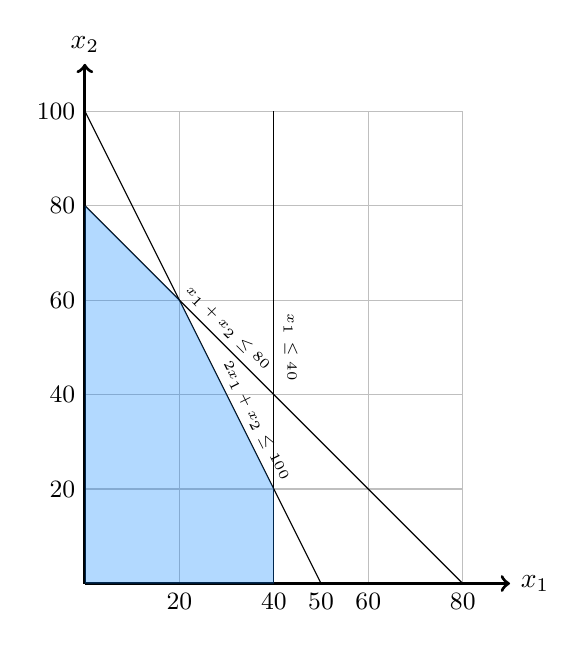
\begin{tikzpicture}[scale=0.06]
		\draw[gray!50, thin, step=20] (0,0) grid (80, 100);
		\draw[very thick,->] (0,0) -- (90, 0) node[right] {$x_1$};
		\draw[very thick,->] (0,0) -- (0, 110) node[above] {$x_2$};
		\foreach \x in {20,40,50,60,80} \draw (\x,0.05) -- (\x,-0.05) node[below] {\small\x};
		\foreach \y in {20,40,60,80,100} \draw (-0.05,\y) -- (0.05,\y) node[left] {\small\y};
		\draw (0,100) -- node[above=5,right=5,sloped] {\tiny$2x_1+x_2\leq100$} (50,0);
		\draw (0,80) -- node[above=5,left=5,sloped] {\tiny$x_1+x_2\leq80$} (80,0);
		\draw (40,100) -- node[above,sloped] {\tiny$x_1\leq40$} (40,0);
		\fill[blue!50!cyan,opacity=0.3] (0,0) -- (0,80) -- (20,60) -- (40,20) -- (40,0) -- cycle;
	\end{tikzpicture}
	\caption[Daerah \textit{feasible}]{Daerah \textit{feasible}}
	\label{fig:daerah_feasible}
\end{figure}

Agar suatu masalah linear programming memiliki solusi optimal, maka daerah feasible harus berbentuk \textit{convex set}. Suatu himpunan titik \(S\) merupakan \textit{convex set} apabila segmen garis yang menghubungkan setiap pasang titik dalam himpunan \(S\) berada dalam himpunan \(S\)~\cite{winston2004operations}. Apabila masalah linear programming memiliki daerah \textit{feasible}, maka daerah tersebut berbentuk \textit{convex set}. Solusi optimal dari masalah tersebut berada pada salah satu \textit{corner point} pada daerah \textit{feasible}. \textit{Extreme point} adalah titik perpotongan antar batasan dan \textit{corner point} adalah \textit{extreme point} yang berada dalam daerah \textit{feasible}. Dengan adanya \textit{corner points}, solusi optimal dapat dicari karena berjumlah terhitung, sehingga tidak perlu memeriksa seluruh kemungkinan solusi masalah yang berjumlah tak hingga. Pada gambar~\ref{fig:corner_points}, titik A, B, C, D, dan E merupakan titik \textit{corner points} yang salah satu di antaranya akan menghasilkan solusi optimal.

\begin{figure}[H]
	\centering
	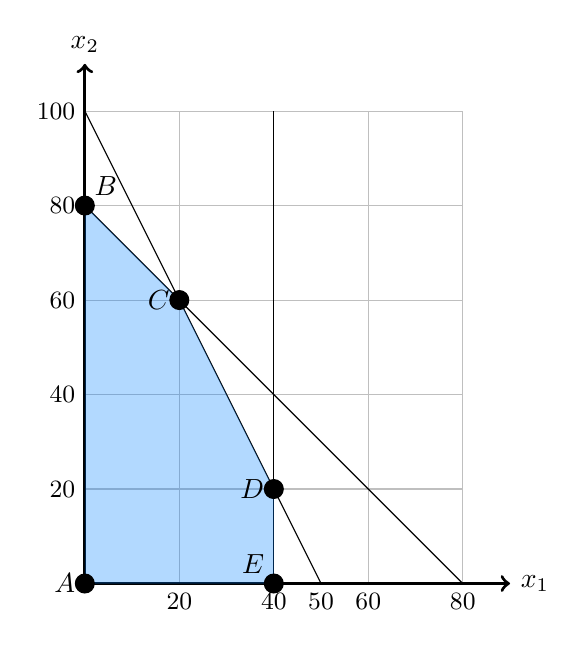
\begin{tikzpicture}[scale=0.06]
		\draw[gray!50, thin, step=20] (0,0) grid (80, 100);
		\draw[very thick,->] (0,0) -- (90, 0) node[right] {$x_1$};
		\draw[very thick,->] (0,0) -- (0, 110) node[above] {$x_2$};
		\foreach \x in {20,40,50,60,80} \draw (\x,0.05) -- (\x,-0.05) node[below] {\small\x};
		\foreach \y in {20,40,60,80,100} \draw (-0.05,\y) -- (0.05,\y) node[left] {\small\y};
		\draw (0,100) -- (50,0);
		\draw (0,80) -- (80,0);
		\draw (40,100) -- (40,0);
		\fill[blue!50!cyan,opacity=0.3] (0,0) -- (0,80) -- (20,60) -- (40,20) -- (40,0) -- cycle;
		\filldraw [black] (0,0) circle (2);
		\filldraw [black] (0,80) circle (2);
		\filldraw [black] (20,60) circle (2);
		\filldraw [black] (40,20) circle (2);
		\filldraw [black] (40,0) circle (2);
		\draw (0,0) node[left] {$A$};
		\draw (0,80) node[above right] {$B$};
		\draw (20,60) node[left] {$C$};
		\draw (40,20) node[left] {$D$};
		\draw (40,0) node[above left] {$E$};
	\end{tikzpicture}
	\caption[\textit{Corner points} pada daerah \textit{feasible}]{Corner points pada daerah \textit{feasible}}
	\label{fig:corner_points}
\end{figure}

Tidak semua masalah linear programming memiliki daerah \textit{feasible}. Apabila batasan-batasan dalam masalah tidak dapat membentuk daerah \textit{feasible}, maka masalah tersebut tidak memiliki solusi apapun, sehingga solusi optimal dari masalah tersebut tidak dapat dicari. Gambar~\ref{fig:daerah_infeasible} menunjukkan contoh masalah linear programming yang tidak memiliki daerah \textit{feasible}.

\begin{figure}[H]
	\centering
	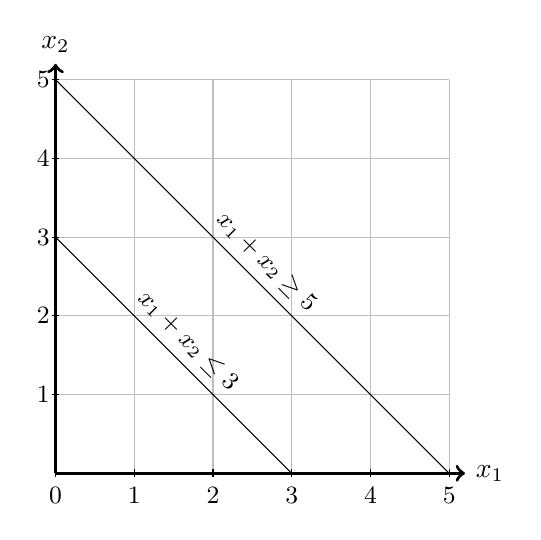
\begin{tikzpicture}
		\draw[gray!50, thin, step=1] (0,0) grid (5,5);
		\draw[very thick,->] (0,0) -- (5.2, 0) node[right] {$x_1$};
		\draw[very thick,->] (0,0) -- (0, 5.2) node[above] {$x_2$};
		\foreach \x in {0,...,5} \draw (\x,0.05) -- (\x,-0.05) node[below] {\small\x};
		\foreach \y in {1,...,5} \draw (-0.05,\y) -- (0.05,\y) node[left] {\small\y};
		\draw (3,0) -- node[above,sloped] {\small $x_1 + x_2 \leq 3$} (0,3);
		\draw (5,0) -- node[above,sloped] {\small $x_1 + x_2 \geq 5$} (0,5);
	\end{tikzpicture}
	\caption[Tidak ada daerah \textit{feasible}]{Tidak ada daerah \textit{feasible}}
	\label{fig:daerah_infeasible}
\end{figure}
	
%Batasan-batasan menghasilkan daerah solusi yang tidak tertutup. Daerah solusi ini memiliki jumlah solusi yang tak terhitung. Gambar~\ref{fig:daerah_solusi_tidak_dibatasi} berikut menggambarkan daerah solusi yang tidak dibatasi.
			
%    	\begin{figure}[H]
%    		\centering
%			\begin{tikzpicture}
%				\draw[gray!50, thin, step=1] (0,0) grid (5,5);
%				\draw[very thick,->] (0,0) -- (5.2, 0) node[right] {$x$};
%				\draw[very thick,->] (0,0) -- (0, 5.2) node[above] {$y$};
%				\foreach \x in {0,...,5} \draw (\x,0.05) -- (\x,-0.05) node[below] {\small\x};
%				\foreach \y in {1,...,5} \draw (-0.05,\y) -- (0.05,\y) node[left] {\small\y};
%				\draw (2,0) -- node[below,sloped] {\small $-2x + 3y \geq -4$} (5,2);
%				\draw (0,1) -- node[above,near end,sloped] {\small $4x - y \geq -1$} (1,5);
%				\fill[blue!50!cyan,opacity=0.3] (0,0) -- (0,1) -- (1,5) -- (5,5) -- (5,2) -- (2,0) -- cycle;
%			\end{tikzpicture}
%			\caption{Daerah solusi yang tidak dibatasi}
%			\label{fig:daerah_solusi_tidak_dibatasi}
%		\end{figure}

\subsection{Bentuk Standar}
Setiap masalah linear programming harus diubah ke dalam bentuk standar sebelum diselesaikan. Berikut ini merupakan struktur dari bentuk standar pada masalah linear programming:
    	
\begin{equation*}
	\setlength\arraycolsep{1.5pt}
	\begin{array}{r r c r c r c r c l}
	    \textit{max}		& \multicolumn{9}{l}{z = c_1x_1 + c_2x_2 + \dots + c_nx_n} \\
		\textit{s.t.} 	& a_{11}x_1 & + & a_{12}x_2 & + & \dots & + & a_{1n}x_n & = & b_1 \\
    						& a_{21}x_1 & + & a_{22}x_2 & + & \dots & + & a_{2n}x_n & = & b_2 \\
                            & \multicolumn{7}{c}{\vdots}                            &   & \vdots \\
                            & a_{m1}x_1 & + & a_{m2}x_2 & + & \dots & + & a_{mn}x_n & = & b_m \\
                            & \multicolumn{9}{l}{x_1\geq0,x_2\geq0,\dots,x_n\geq0}
	\end{array}
\end{equation*}

Bentuk standar masalah linear programming terdiri dari $n$ buah variabel keputusan $x$ dan $m$ buah persamaan batasan. Setiap batasan dalam bentuk standar harus dalam bentuk persamaan dan batasan non-negatif diberlakukan untuk setiap varibel keputusan. Bentuk standar linear programming dapat dinyatakan dalam notasi matriks seperti berikut ini:
        
\begin{equation*}
	\begin{array}{r l}
    	\textit{max}   & z=C^Tx \\
        \textit{s.t.} & Ax=b \textit{ and } x\geq0
	\end{array}    
\end{equation*}

dengan

%\begin{equation*}
%	c = \left[
%	\begin{array}{c}
%    	c_1\\
%    	c_2\\
%    	\vdots\\
%   	c_n
%	\end{array}
%	\right]    
%\end{equation*}

\begin{equation*}
	A = \left[
	\begin{array}{c c c c}
    	a_{11} & a_{12} & \dots & a_{1n}\\
    	a_{21} & a_{22} & \dots & a_{2n}\\
    	\vdots & \vdots & & \vdots\\
    	a_{m1} & a_{m2} & \dots & a_{mn}
	\end{array}
	\right]    
\end{equation*}

\begin{equation*}
	x = \left[
	\begin{array}{c}
    	x_1\\
    	x_2\\
    	\vdots\\
    	x_n
	\end{array}
	\right]    
\end{equation*}

\begin{equation*}
	b = \left[
	\begin{array}{c}
    	b_1\\
    	b_2\\
    	\vdots\\
    	b_m
	\end{array}
	\right]    
\end{equation*}

Pada notasi matriks, $x$ menunjukkan matriks kolom berdimensi $n$, $C^T$ menunjukkan matriks baris berdimensi $n$, $A$ menunjukkan matriks berdimensi $m\times n$, dan $b$ menunjukkan matriks kolom berdimensi $m$. Matriks $x\geq0$ menunjukkan batasan non-negatif untuk setiap variabel keputusan $x_i$. Untuk mengubah masalah linear programming ke bentuk standar, maka setiap batasan perlu diubah. Perubahan batasan dibedakan berdasarkan tandanya, yaitu sebagai berikut:
		
		\begin{itemize}
			\item \textbf{Batasan dengan tanda pertidaksamaan \(\leq\)}\\
				Pertidaksamaan pada batasan ini diubah ke dalam bentuk persamaan dengan menambahkan variabel positif \(s_i\) yang disebut \textit{slack} pada sisi kiri. Lalu ditambahkan batasan non-negatif untuk variabel \textit{slack} tersebut. Contoh:
				
				\begin{equation*}
					x_1 + 2x_2 \leq 40
				\end{equation*}
				
				diubah menjadi
				
				\begin{equation*}
					\begin{split}
						x_1 + 2x_2 + s_1 &= 40\\
						s_1 &\geq 0
					\end{split}
				\end{equation*}
			
			\item \textbf{Batasan dengan tanda pertidaksamaan \(\geq\)}\\			
				Pertidaksamaan pada batasan ini diubah ke dalam bentuk persamaan dengan menambahkan variabel negatif \(e_i\) yang disebut \textit{excess} pada sisi kiri. Lalu ditambahkan batasan non-negatif untuk variabel \textit{excess} tersebut. Contoh:
				
				\begin{equation*}
					x_1 + 2x_2 \geq 40
				\end{equation*}
				
				diubah menjadi
				
				\begin{equation*}
					\begin{split}
						x_1 + 2x_2 - e_1 &= 40\\
						e_1 &\geq 0
					\end{split}
				\end{equation*}				
		\end{itemize}
		
%	\item Mengsubtitusi variabel bebas
	
%		Apabila terdapat variabel bebas \(x_i\), maka subtitusikan setiap variabel tersebut dengan 2 variabel pengganti \(u_i\) dan \(v_i\) sehingga \(x_i = u_i - v_i\). Lalu tambahkan tanda pembatas tidak negatif untuk variabel \(u_i\) dan \(v_i\). Contoh:
		
%		\begin{equation*}
%			\begin{array}{r r c r c l}
%				\text{maximize} & \multicolumn{5}{l}{z = x_1 + x_2}\\
%				\text{subject to} & 2x_1 & + & x_2 & \leq & 4\\
%									& \multicolumn{3}{r}{x_1} & \geq & 0\\
%			\end{array}
%		\end{equation*}
		
%		dengan
		
%		\begin{equation*}
%			x_2 = u_2 - v_2
%		\end{equation*}
		
%		menjadi
		
%		\begin{equation*}
%			\begin{array}{r r c r c r c l}
%				\text{maximize} & \multicolumn{7}{l}{z = x_1 + u_2 - v_2}\\
%				\text{subject to} & 2x_1 & + & u_2 & - & v_2 & \leq & 4\\
%									& \multicolumn{5}{r}{x_1} & \geq & 0\\
%									& \multicolumn{5}{r}{u_2} & \geq & 0\\
%									& \multicolumn{5}{r}{v_2} & \geq & 0\\
%			\end{array}
%		\end{equation*}
%\end{enumerate}

\subsection{Variabel Basis dan Non-basis}
Masalah linear programming \(Ax = b\) terdiri dari \(m\) buah persamaan batasan dan \(n\) buah variabel keputusan. Masalah ini memiliki solusi yang disebut dengan solusi basis apabila membuat \((n - m)\) buah variabel keputusan bernilai 0 dan menyelesaikan \(m\) buah variabel keputusan lainnya. Sebanyak \((n - m)\) buah variabel yang dibuat bernilai 0 disebut dengan variabel non-basis. Sedangkan \(m\) buah variabel lainnya disebut dengan variabel basis. Berikut contoh sistem persamaan linear:
%Variabel basis merupakan variabel yang diselesaikan setelah membuat variabel lain menjadi variabel non basis. 

\begin{equation*}
	\setlength\arraycolsep{1.5pt}
	\begin{array}{r c r c r c l}
		x_1 &+ &x_2 &  &    &= &3\\
		    &- &x_2 &+ &x_3 &= &-1
	\end{array}
\end{equation*}

Pada sistem persamaan linear di atas, dipilih sebanyak 3 - 2 = 1 (3 variabel dan 2 persamaan) buah variabel yang akan menjadi variabel non basis. Jika himpunan variabel non basis NBV = \(\{x_3\}\), maka himpunan variabel basis BV = \(\{x_1, x_2\}\). Solusi dari sistem persamaan tersebut dapat dicari dengan membuat setiap variabel NBV menjadi variabel non basis dan menyelesaikan variabel BV.

\begin{equation*}
	\setlength\arraycolsep{1.5pt}
	\begin{array}{r c r c r c l}
		x_1 &+ &x_2 &  &    &= &3\\
		    &- &x_2 &+ &0 &= &-1
	\end{array}
\end{equation*}

Pada persamaan di atas didapatkan nilai \(x_1\) = 2 dan \(x_2\) = 1. Dengan demikian didapatkan solusi basis dengan nilai \(x_1\) = 2, \(x_2\) = 1, dan \(x_3\) = 0.

\subsection{Metode Simplex}
Metode simplex merupakan metode yang digunakan untuk menyelesaikan masalah linear programming. Berikut ini merupakan langkah-langkah metode simplex:
\begin{enumerate}
	\item Mengubah masalah linear programming ke dalam bentuk standar
	\item Mencari \textit{basic feasible solution} (\textit{bfs}) dari bentuk standar.
	\item Memeriksa apakah \textit{bfs} pada saat ini sudah optimal.
	\item Apabila \textit{bfs} belum optimal, tentukan variabel non-basis mana yang akan menjadi variabel basis dan tentukan variabel basis mana yang akan menjadi variabel non-basis dengan tujuan mencari \textit{bfs} baru yang dapat meningkatkan nilai fungsi objektif.
	\item Lakukan Operasi Baris Elementer (OBE) untuk mencari \textit{bfs} baru yang dapat meningkatkan nilai fungsi objektif. Lanjut ke langkah 3.
\end{enumerate}

Fungsi objektif yang berbentuk
\begin{equation*}
	z = c_1x_1 + c_2x_2 + \dots + c_nx_n
\end{equation*}
ditulis dalam bentuk
\begin{equation*}
	z - c_1x_1 - c_2x_2 - \dots - c_nx_n = 0
\end{equation*}
Bentuk fungsi objektif ini disebut sebagai baris 0.

Untuk memahami penyelesaian masalah linear programming menggunakan metode simplex, akan digunakan sebuah contoh masalah linear programming sebagai berikut:
\begin{equation*}
	\setlength\arraycolsep{1.5pt}
	\begin{array}{r r c r c r c l}
		\textit{max } &\multicolumn{7}{l}{z = 60x_1 + 30x_2 + 20x_3}\\
		\textit{s.t.} &8x_1 &+ &6x_2 &+ &x_3 &\leq &48\\
		&4x_1 &+ &2x_2 &+ &1.5x_3 &\leq &20\\
		&2x_1 &+ &1.5x_2 &+ &0.5x_3 &\leq &8\\
		&&&x_2 &&&\leq &5\\
		&&&&&x_1 &\geq &0\\
		&&&&&x_2 &\geq &0\\
		&&&&&x_3 &\geq &0\\
	\end{array}
\end{equation*}

Langkah pertama adalah mengubah masalah ke bentuk standar, sehingga masalah ini dalam bentuk standar adalah sebagai berikut:

\begin{equation*}
	\setlength\arraycolsep{1.5pt}
	\begin{array}{r r c r c r c r c r c r c r c l}
		\textit{max } &\multicolumn{15}{l}{z = 60x_1 + 30x_2 + 20x_3}\\
		\textit{s.t.} &8x_1 &+ &6x_2 &+ &x_3 &+ &s_1 &&&&&&&= &48\\
		&4x_1 &+ &2x_2 &+ &1.5x_3 &&&+ &s_2 &&&&&= &20\\
		&2x_1 &+ &1.5x_2 &+ &0.5x_3 &&&&&+ &s_3 &&&= &8\\
		&&&x_2 && &&&&&&&+ &s_4 &= &5\\
		\multicolumn{14}{r}{x_1, x_2, x_3, s_1, s_2, s_3, s_4} &\geq &0\\
	\end{array}
\end{equation*}

Masalah dalam bentuk standar ini disajikan dalam bentuk tabel simplex seperti pada tabel~\ref{tab:tabel_simplex_0}. Pada tabel ini, baris pertama (baris 0) merupakan baris bagi fungsi objektif dan baris lainnya merupakan baris bagi variabel basis. Pada tabel simplex pertama, variabel basis terdiri dari variabel \textit{slack} dan variabel \textit{excess}.

\begin{center}
	\captionof{table}{Tabel simplex 0}
	\label{tab:tabel_simplex_0}
	$
	\begin{array}{|r r r r r r r r|c|r c l|}
		\hline
		z & x_1 & x_2 & x_3 & s_1 & s_2 & s_3 & s_4 & \textit{rhs} & \multicolumn{3}{c|}{\textit{basic variable}}\\
		\hline
		1 & -60 & -30 & -20 & 0 & 0 & 0 & 0 & 0 & z & = & 0\\
		0 & 8 & 6 & 1 & 1 & 0 & 0 & 0 & 48 & s_1 & = & 48\\
		0 & 4 & 2 & 1.5 & 0 & 1 & 0 & 0 & 20 & s_2 & = & 20\\
		0 & 2 & 1.5 & 0.5 & 0 & 0 & 1 & 0 & 8 & s_3 & = & 8\\
		0 & 0 & 1 & 0 & 0 & 0 & 0 & 1 & 5 & s_4 & = & 5\\
		\hline
	\end{array}
	$
\end{center}

Kolom \textit{right hand side} (\textit{rhs}) menunjukkan nilai pada ruas kanan (nilai di sebelah kanan tanda sama dengan). Kolom \textit{basic variable} menunjukkan variabel basis beserta dengan nilainya. Kolom \textit{basic variable} juga menunjukkan solusi basis \textit{feasible} (\textit{bfs}) sehingga tabel~\ref{tab:tabel_simplex_0} menunjukkan \textit{bfs} dengan nilai \(z=0, x_1=0, x_2=0, x_3=0, s_1=48, s_2=20, s_3=8, \text{ dan } s_4=5\). Setiap variabel yang tidak berada di dalam kolom \textit{basic variable} menandakan bahwa variabel-variabel tersebut merupakan variabel non-basis sehingga bernilai 0.

Langkah selanjutnya adalah memeriksa apakah \textit{bfs} sudah optimal. Pada langkah ini akan diperiksa apakah terdapat variabel negatif (untuk kasus maksimasi) pada baris 0 di setiap kolom variabel. Pada tabel~\ref{tab:tabel_simplex_0}, masih terdapat variabel negatif, yaitu pada variabel \(x_1, x_2, \text{ dan } x_3\).
Hal ini menunjukkan bahwa \textit{bfs} saat ini masih belum optimal.

Apabila \textit{bfs} pada saat ini masih belum optimal, maka perlu dilakukan proses \textit{pivotting}. Proses \textit{pivotting} adalah proses penukaran variabel basis dengan variabel non-basis. Variabel yang akan menjadi variabel basis disebut dengan \textit{entering variable} dan variabel basis yang akan digantikan disebut dengan \textit{leaving variable}. \textit{Entering variable} dipilih dengan cara memilih variabel yang bernilai paling negatif pada baris 0. Untuk mencari \textit{leaving variable} perlu dilakukan tes rasio. Tes rasio membandingkan nilai pada nilai \textit{rhs} dengan nilai pada kolom \textit{entering variable}. Tes rasio hanya perlu dilakukan pada baris yang variable pada kolom \textit{entering variable} bernilai lebih besar dari 0. \textit{Leaving variable} dipilih dengan cara memilih variabel pada baris yang menghasilkan rasio terkecil. Perpotongan antara kolom \textit{entering variable} dengan baris \textit{leaving variable}.merupakan suatu elemen yang disebut \textit{pivot element}.

Dalam contoh masalah, \textit{bfs} pada saat ini masih belum optimal, sehingga perlu dilakukan proses \textit{pivotting}. Variabel \(x_1\) akan menjadi \textit{entering variable} karena bernilai paling negatif pada baris 0. Setelah dilakukan tes rasio sesuai, variabel \(s_3\) menjadi \textit{leaving variable} karena memiliki hasil tes rasio terkecil. Tes rasio untuk \textit{bfs} baru pada contoh masalah dapat dilihat pada tabel~\ref{tab:tabel_pivotting_1}.

\begin{center}
	\captionof{table}{Tabel \textit{pivotting} 1}
	\label{tab:tabel_pivotting_1}
	$
	\begin{array}{|r r r r r r r r|c|r c l|r c l|}
		\hline
		z & x_1 & x_2 & x_3 & s_1 & s_2 & s_3 & s_4 & \textit{rhs} & \multicolumn{3}{c|}{\textit{basic variable}} & \multicolumn{3}{c|}{\textit{ratio}}\\
		\hline
		1 & -60 & -30 & -20 & 0 & 0 & 0 & 0 & 0 & z & = & 0 &&&\\
		0 & 8 & 6 & 1 & 1 & 0 & 0 & 0 & 48 & s_1 & = & 48 & \nicefrac{48}{8} & = & 6\\
		0 & 4 & 2 & 1.5 & 0 & 1 & 0 & 0 & 20 & s_2 & = & 20 & \nicefrac{20}{4} & = & 5\\
		0 & \encircle{2} & 1.5 & 0.5 & 0 & 0 & 1 & 0 & 8 & s_3 & = & 8 & \nicefrac{8}{2} & = & 4\\
		0 & 0 & 1 & 0 & 0 & 0 & 0 & 1 & 5 & s_4 & = & 5 &&&\\
		\hline
	\end{array}
	$
\end{center}

Setelah menentukan \textit{entering variable} dan \textit{leaving variable}, akan dilakukan OBE. OBE dilakukan untuk membuat \textit{entering variable} menjadi variabel basis, sehingga \textit{entering variable} pada baris {leaving variable} bernilai 1 dan variabel lain pada kolom \textit{entering variable} bernilai 0. Setelah OBE dilakukan, baris \textit{leaving variable} akan memiliki \textit{entering variable} sebagai variabel basis.

Dalam contoh masalah, telah ditentukan \textit{entering variable} dan \textit{leaving variable}. Variabel yang menjadi \textit{entering variable} adalah variabel \(x_1\) yang berada pada kolom \(x_1\). Variabel yang menjadi \textit{Leaving variable} adalah variabel \(s_3\) yang berada pada baris 3. Dengan OBE, \textit{entering variable} pada baris 3 akan dibuat bernilai 1 dan variabel lain pada kolom \textit{entering variable} akan dibuat bernilai 0. Berikut ini urutan OBE yang dilakukan:
\begin{enumerate}
	\item Untuk mendapatkan variabel \(x_1\) bernilai 1 pada baris 3, maka baris 3' baru dapat dibentuk dari baris 3 lama yang dikalikan dengan \(\nicefrac{1}{2}\).\\
	\begin{equation*}
		\frac{1}{2}R_3 \rightarrow R_3'
	\end{equation*}
	sehingga baris 3' baru menjadi
	\begin{equation*}
		x_1 + 0.75x_2 + 0.25x_3 + 0.5s_3 = 4
	\end{equation*}
	
	\item Untuk mendapatkan variabel \(x_1\) bernilai 0 pada baris 0, maka baris 0' baru dapat dibentuk dari baris 3' baru yang dikalikan 60 dan ditambahkan dengan baris 0 lama.\\
	\begin{equation*}
		60R_3 + R_0 \rightarrow R_0'
	\end{equation*}
	sehingga baris 0' baru menjadi
	\begin{equation*}
		z + 15x_2 - 5x_3 + 30s_3 = 240
	\end{equation*}

	\item Untuk mendapatkan variabel \(x_1\) bernilai 0 pada baris 1, maka baris 1' baru dapat dibentuk dari baris 3' baru yang dikalikan -8 dan ditambahkan dengan baris 1 lama.\\
	\begin{equation*}
		-8R_3 + R_1 \rightarrow R_1'
	\end{equation*}
	sehingga baris 1' baru menjadi
	\begin{equation*}
		-x_3 + s_1 - 4s_3 = 16
	\end{equation*}

	\item Untuk mendapatkan variabel \(x_1\) bernilai 0 pada baris 2, maka baris 2' baru dapat dibentuk dari baris 3' baru yang dikalikan -4 dan ditambahkan dengan baris 2 lama.\\
	\begin{equation*}
		-4R_2 + R_2 \rightarrow R_2'
	\end{equation*}
	sehingga baris 2' baru menjadi
	\begin{equation*}
		-x_2 + 0.5x_3 + s_2 - 2s_3 = 4
	\end{equation*}
\end{enumerate}

Karena nilai \(x_1\) bernilai 0 pada baris 4, maka tidak perlu dilakukan OBE pada baris 4, sehingga baris 4' baru sama dengan baris 4 lama. \textit{Entering variable} menggantikan \textit{leaving variable} pada baris 3 sehingga \(x_1\) menjadi variabel basis yang baru. Setelah melakukan OBE, maka didapatkan tabel simplex baru seperti pada tabel~\ref{tab:tabel_simplex_1} yang menunjukkan \textit{bfs} dengan nilai \(z=240, x_1=4, x_2=0, x_3=0, s_1=16, s_2=4, s_3=0, \text{ dan } s_4=5\).

\begin{center}
	\captionof{table}{Tabel simplex 1}
	\label{tab:tabel_simplex_1}
	$
	\begin{array}{|r r r r r r r r|c|r c l|}
		\hline
		z & x_1 & x_2 & x_3 & s_1 & s_2 & s_3 & s_4 & \textit{rhs} & \multicolumn{3}{c|}{\textit{basic variable}}\\
		\hline
		1 & 0 & 15 & -5 & 0 & 0 & 30 & 0 & 240 & z & = & 240\\
		0 & 0 & 0 & -1 & 1 & 0 & -4 & 0 & 16 & s_1 & = & 16\\
		0 & 0 & -1 & 0.5 & 0 & 1 & -2 & 0 & 4 & s_2 & = & 4\\
		0 & 1 & 0.75 & 0.25 & 0 & 0 & 0.5 & 0 & 4 & x_1 & = & 4\\
		0 & 0 & 1 & 0 & 0 & 0 & 0 & 1 & 5 & s_4 & = & 5\\
		\hline
	\end{array}
	$
\end{center}

Setelah mendapatkan tabel simplex~\ref{tab:tabel_simplex_1}, langkah selanjutnya adalah memeriksa apakah \textit{bfs} pada iterasi ini sudah optimal. Pada baris 0, terdapat nilai negatif, yaitu pada variabel \(x_3\), sehingga \textit{bfs} ini belum optimal. Maka  langkah selanjutnya adalah mencari \textit{entering variable} dan \textit{leaving variable}. \textit{Entering variable} didapatkan dengan memilih variabel yang bernilai paling negatif pada baris 0, yaitu variabel \(x_3\). \textit{Leaving variable} didapatkan dengan mencari rasio terkecil dari hasil tes rasio. Tes rasio dapat dilihat pada tabel~\ref{tab:tabel_pivotting_2}. Variabel \(s_2\) menghasilkan hasil tes rasio terkecil, sehingga variabel \(s_2\) menjadi \textit{leaving variable}.

\begin{center}
	\captionof{table}{Tabel \textit{pivotting} 2}
	\label{tab:tabel_pivotting_2}
	$
	\begin{array}{|r r r r r r r r|c|r c l|r c l|}
		\hline
		z & x_1 & x_2 & x_3 & s_1 & s_2 & s_3 & s_4 & \textit{rhs} & \multicolumn{3}{c|}{\textit{basic variable}} & \multicolumn{3}{c|}{\textit{ratio}}\\
		\hline
		1 & 0 & 15 & -5 & 0 & 0 & 30 & 0 & 240 & z & = & 240 &&&\\
		0 & 0 & 0 & -1 & 1 & 0 & -4 & 0 & 16 & s_1 & = & 16 &&&\\
		0 & 0 & -1 & \encircle{0.5} & 0 & 1 & -2 & 0 & 4 & s_2 & = & 4 & \nicefrac{4}{0.5} & = & 8\\
		0 & 1 & 0.75 & 0.25 & 0 & 0 & 0.5 & 0 & 4 & x_1 & = & 4 & \nicefrac{4}{0.25} & = & 16\\
		0 & 0 & 1 & 0 & 0 & 0 & 0 & 1 & 5 & s_4 & = & 5 &&&\\
		\hline
	\end{array}
	$
\end{center}

Selanjutnya dilakukan OBE untuk membuat \textit{entering variable} \(x_3\) menjadi variabel basis. Berikut ini urutan OBE yang dilakukan:
\begin{enumerate}
	\item Untuk mendapatkan variabel \(x_3\) bernilai 1 pada baris 2, maka baris 2'' baru dapat dibentuk dari baris 2' lama yang dikalikan dengan 2.\\
	\begin{equation*}
		2R_2' \rightarrow R_2''
	\end{equation*}
	sehingga baris 2'' baru menjadi
	\begin{equation*}
		-2x_2 + x_3 + 2s_2 - 4s_3 = 8
	\end{equation*}
	
	\item Untuk mendapatkan variabel \(x_3\) bernilai 0 pada baris 0, maka baris 0'' baru dapat dibentuk dari baris 2'' baru yang dikalikan 5 dan ditambahkan dengan baris 0' lama.\\
	\begin{equation*}
		5R_2'' + R_0' \rightarrow R_0''
	\end{equation*}
	sehingga baris 0'' baru menjadi
	\begin{equation*}
		z + 5x_2 + 10s_2 + 10s_3 = 280
	\end{equation*}
	
	\item Untuk mendapatkan variabel \(x_3\) bernilai 0 pada baris 1, maka baris 1'' baru dapat dibentuk dari baris 2'' baru yang ditambahkan dengan baris 1' lama.\\
	\begin{equation*}
		R_2'' + R_1' \rightarrow R_1''
	\end{equation*}
	sehingga baris 1'' baru menjadi
	\begin{equation*}
		-2x_2 + s_1 + 2s_2 - 8s_3 = 24
	\end{equation*}
	
	\item Untuk mendapatkan variabel \(x_3\) bernilai 0 pada baris 3, maka baris 3'' baru dapat dibentuk dari baris 2'' baru yang dikalikan \(-\nicefrac{1}{4}\) dan ditambahkan dengan baris 3' lama.\\
	\begin{equation*}
		-\frac{1}{4}R_2'' + R_3' \rightarrow R_3''
	\end{equation*}
	sehingga baris 3'' baru menjadi
	\begin{equation*}
		x_1 + 1.25x_2 - 0.5s_2 + 1.5s_3 = 2
	\end{equation*}
\end{enumerate}

Variabel \(x_3\) sudah bernilai 0 pada baris 4, maka baris 4 yang baru sama dengan baris 4 yang lama. Variabel \(x_3\) menjadi variabel basis baru yang menggantikan variabel \(s_2\). Setelah melakukan OBE, didapatkan tabel simplex~\ref{tab:tabel_simplex_2} yang menunjukkan \textit{bfs} dengan nilai \(z=280, x_1=2, x_2=0, x_3=8, s_1=24, s_2=0, s_3=0, \text{ dan } s_4=5\).

\begin{center}
	\captionof{table}{Tabel simplex 2}
	\label{tab:tabel_simplex_2}
	$
	\begin{array}{|r r r r r r r r|c|r c l|}
		\hline
		z & x_1 & x_2 & x_3 & s_1 & s_2 & s_3 & s_4 & \textit{rhs} & \multicolumn{3}{c|}{\textit{basic variable}}\\
		\hline
		1 & 0 & 5 & 0 & 0 & 10 & 10 & 0 & 280 & z & = & 280\\
		0 & 0 & -2 & 0 & 1 & 2 & -8 & 0 & 24 & s_1 & = & 24\\
		0 & 0 & -2 & 1 & 0 & 2 & -4 & 0 & 8 & x_3 & = & 8\\
		0 & 1 & 1.25 & 0 & 0 & -0.5 & 1.5 & 0 & 2 & x_1 & = & 2\\
		0 & 0 & 1 & 0 & 0 & 0 & 0 & 1 & 5 & s_4 & = & 5\\
		\hline
	\end{array}
	$
\end{center}

Langkah selanjutnya adalah memeriksa apakah \textit{bfs} saat ini sudah optimal. Pada baris 0, tidak ditemukan variabel bernilai negatif, sehingga \textit{bfs} pada tahap ini sudah optimal. Dengan demikian masalah ini memiliki solusi optimal bernilai 280 dengan variabel \(x_1=2, x_2=0, x_3=8, \text{ dan } x_4 = 0\).

\subsection{Metode Simplex 2}

Metode simplex merupakan metode yang digunakan untuk mencari solusi optimal dari masalah linear programming. Metode simplex bekerja secara beriterasi dengan menghasilkan solusi yang mendekati optimal pada setiap iterasinya. Iterasi ini akan dilakukan hingga tidak ditemukannya solusi yang lebih optimal. Berikut contoh masalah linear programming:

\begin{equation*}
	\begin{array}{r c c c c l}
		\text{maximize}   & 3x_1 & + & 2x_2 \\
		\text{subject to} & 2x_1 & + & x_2  & \leq & 18 \\
        					& 2x_1 & + & 3x_2 & \leq & 42 \\
                           	& 3x_1 & + & x_2  & \leq & 24 \\
                           	& \multicolumn{5}{l}{x_1\geq0,x_2\geq0} \\
	\end{array}
\end{equation*}
        
Langkah-langkah untuk menyelesaikan maslaah linear programming dengan menggunakan metode simplex:

\begin{enumerate}
	\item Mengubah masalah ke dalam bentuk standar
	
        Masalah linear programming diubah ke bentuk standar sesuai dengan langkah-langkah yang sudah dibahas sebelumnya.
        
        Berikut contoh masalah linear programming yang sudah diubah ke bentuk standar:
        
	    \begin{equation*}
			\begin{array}{r c c c c c c c c c c l}
    	    	\text{maximize}   & 3x_1 & + & 2x_2 & + & 0x_3 & + & 0x_4 & + & 0x_5\\
	            \text{subject to} & 2x_1 & + & x_2  & + & x_3 &   &       &   &       & = & 18 \\
                        	   		& 2x_1 & + & 3x_2 &   &       & + & x_4 &   &       & = & 42 \\
                    	       		& 3x_1 & + & x_2  &   &       &   &       & + & x_5 & = & 24 \\
                	           		& \multicolumn{11}{l}{x_1\geq0,x_2\geq0,x_3\geq0,x_4\geq0,x_5\geq0} \\
        	\end{array}
		\end{equation*}
			
	\item Membuat tabel \textit{simplex}\\
		Tabel~\ref{tab:kerangka_tabel_simplex} merupakan kerangka tabel simplex yang terdiri dari 4 kolom utama, yaitu kolom basis, kolom $z$, kolom variabel non basis, dan kolom ruas kanan/rhs (\textit{right hand side}). Pada awalnya, baris $z$ berisi nilai negatif dari konstanta variabel pada fungsi tujuan dan $m$ baris berikutnya berisi konstanta variabel pada setiap persamaan batasan. $m$ baris terkahir ini diidentifikasikan sebagai baris basis.
        	
		\begin{table}[H]
			\centering
			\caption{Kerangka tabel simplex}
			\label{tab:kerangka_tabel_simplex}
			\begin{tabular}{|c|c|c c c c |c|}
				\hline
				basic & $z$ & $x_1$ & $x_2$ & \dots & $x_n$ & rhs \\
				\hline
				$z$ & 1 & $-c_1$ & $-c_2$ & \dots & $-c_n$ & 0 \\
				\hline
				$x_{n+1}$ & 0 & $a_{11}$ & $a_{12}$ & \dots & $a_{1n}$ & $b_1$ \\
				$x_{n+2}$ & 0 & $a_{21}$ & $a_{22}$ & \dots & $a_{2n}$ & $b_2$ \\
				\vdots & \vdots & \vdots & \vdots & \vdots & \vdots & \vdots \\
				$x_{n+m}$ & 0 & $a_{m1}$ & $a_{m2}$ & \dots & $a_{mn}$ & $b_m$ \\
				\hline
			\end{tabular}
		\end{table}
			
		Tabel~\ref{tab:contoh_simplex_awal} berikut adalah tabel simplex awal untuk contoh masalah linear programming.
			
		\begin{table}[H]
			\centering
			\caption{Tabel simplex awal}
			\label{tab:contoh_simplex_awal}
			\begin{tabular}{|c|c|c c c c c|c|}
				\hline
				basic & $z$ & $x_1$ & $x_2$ & $x_3$ & $x_4$ & $x_5$ & rhs \\
				\hline
				$z$ & 1 & -3 & -2 & 0 & 0 & 0 & 0 \\
				\hline
				$x_3$ & 0 & 2 & 1 & 1 & 0 & 0 & 18\\
				$x_4$ & 0 & 2 & 3 & 0 & 1 & 0 & 42\\
				$x_5$ & 0 & 3 & 1 & 0 & 0 & 1 & 24\\
				\hline
			\end{tabular}
		\end{table}

	\item Mengecek solusi optimal
	
    	Apabila pada baris $z$ tidak terdapat variabel dengan nilai negatif, maka solusi optimal sudah ditemukan dan menandakan akhir dari iterasi. Solusi optimal terdapat pada setiap rhs dari setiap baris basis. Jika masih terdapat variabel dengan nilai negatif, maka langkah selanjutnya adalah melakukan proses \textit{pivoting}.

		Pada Tabel~\ref{tab:contoh_simplex_awal}, terdapat nilai negatif di baris $z$, yaitu pada variabel $x_1$ dan $x_2$. Sehingga dilanjutkan ke proses \textit{pivoting}.

	\item Melakukan proses \textit{pivoting}
		
    	Proses \textit{pivoting} merupakan proses penukaran satu variabel basis dengan satu variabel non basis. Variabel basis yang akan digantikan (keluar dari baris basis) disebut dengan \textit{leaving variable} dan variabel non basis yang akan menggantikan (masuk ke baris basis) disebut \textit{entering variable}. Ketentuan dalam pemilihan variabel yang akan ditukar adalah sebagai berikut:

		\begin{itemize}
    		\item \textit{Entering variable} dipilih berdasarkan nilai terkecil dalam baris $z$. Kolom dari \textit{entering variable} akan menjadi kolom pivot (\textit{pivot column}).
    		
    		\item \textit{Leaving variable} dipilih berdasarkan rasio tidak negatif terkecil antara rhs dengan nilai pada kolom pivot. Baris dari \textit{leaving variable} akan menjadi baris pivot (\textit{pivot row}).

			\item Pivot merupakan nilai yang berada di perpotongan kolom pivot dan baris pivot.
    	\end{itemize}

    	Pada Tabel~\ref{tab:contoh_simplex_pemilihan_pivot}, $x_1$ menjadi \textit{entering variabel} karena bernilai paling kecil di baris $z$, yaitu $-3$. Sedangkan baris basis $x_5$ menjadi \textit{leaving variable} karena nilai rasionya yang paling kecil, yaitu 8. Perpotongan baris pivot dan kolom pivot menghasilkan pivot bernilai $3$.

    	\begin{table}[H]
    		\centering
			\caption{Pemilihan pivot}
    		\label{tab:contoh_simplex_pemilihan_pivot}			
			\begin{tabular}{c|c|c|c c c c c|c|c}
				\multicolumn{3}{c}{} & \multicolumn{6}{l}{\textit{pivot column}}\\
				\multicolumn{3}{c}{} & $\downarrow$ & \multicolumn{5}{c}{}\\
				\cline{2-9}
				& basic & $z$ & $x_1$ & $x_2$ & $x_3$ & $x_4$ & $x_5$ & rhs & ratio: \\
				\cline{2-9}
				& $z$ & 1 & -3 & -2 & 0 & 0 & 0 & 0 & $\frac{rhs_i}{pivotCol_{i}}$ \\
				\cline{2-9}
				& $x_3$ & 0 & 2 & 1 & 1 & 0 & 0 & 18 & $\frac{18}{2}=9$\\
				& $x_4$ & 0 & 2 & 3 & 0 & 1 & 0 & 42 & $\frac{42}{2}=21$\\
				\textit{pivot row} $\rightarrow$ & $x_5$ & 0 & \encircle{3} & 1 & 0 & 0 & 1 & 24 & $\frac{24}{3}=8$\\
				\cline{2-9}
			\end{tabular}
		\end{table}
    		
    \item Memperbaharui tabel simplex
    
		Setiap nilai pada baris basis baru akan dibagi dengan nilai pivot sebelumnya. Sedangkan nilai pada baris basis lainnya dikurangi dengan hasil perkalian antara nilai kolom pivot yang bersangkutan dengan nilai baru pada baris pivot yang bersangkutan. Setelah diperbaharui, langkah selanjutnya adalah kembali pada pengecekan solusi optimal.

		Pada Tabel~\ref{tab:contoh_simplex_pembaharuan_tabel_simplex}, $x_1$ menjadi baris basis yang baru. Setiap nilai pada baris tersebut dibagi dengan nilai pivot sebelumnya yang bernilai $3$. Setiap nilai pada baris basis lainnya diubah sesuai dengan ketentuan yang sudah dibahas sebelumnya.
			
		\begin{table}[H]
			\centering
			\caption{Pembaharuan tabel simplex}
			\label{tab:contoh_simplex_pembaharuan_tabel_simplex}
			\small
			\begin{tabular}{|c|c|c @{\hspace{0.2cm}}c @{\hspace{0.2cm}}c @{\hspace{0.2cm}}c @{\hspace{0.2cm}}c|c|c}
				\hline
				basic & $z$ & $x_1$ & $x_2$ & $x_3$ & $x_4$ & $x_5$ & rhs \\
				\hline
				$z$ & 1 & $-3-(-3\times\frac{3}{3})$ & $-2-(-3\times\frac{1}{3})$ & $0-(-3\times0)$ & $0-(-3\times0)$ & $0-(-3\times\frac{1}{3})$ & $0-(-3\times\frac{24}{3})$ \\
				\hline
				$x_3$ & 0 & $2-(2\times\frac{3}{3})$ & $1-(2\times\frac{1}{3})$ & $1-(2\times0)$ & $0-(2\times0)$ & $0-(2\times\frac{1}{3})$ & $18-(2\times\frac{24}{3})$ \\
				$x_4$ & 0 & $2-(2\times\frac{3}{3})$ & $3-(2\times\frac{1}{3})$ & $0-(2\times0)$ & $1-(2\times0)$ & $0-(2\times\frac{1}{3})$ & $42-(2\times\frac{24}{3})$ \\
				$x_1$ & 3 & $\frac{3}{3}$ & $\frac{1}{3}$ & 0 & 0 & $\frac{1}{3}$ & $\frac{24}{3}$ \\
				\hline
			\end{tabular}
		\end{table}
			
		Tabel~\ref{tab:contoh_simplex_iterasi_1} berikut merupakan tabel simplex pada akhir iterasi ke-1:
			
		\begin{table}[H]
			\centering
			\caption{Tabel simplex iterasi ke-1}
			\label{tab:contoh_simplex_iterasi_1}
			\begin{tabular}{|c|c|c c c c c|c|c}
				\hline
				basic & $z$ & $x_1$ & $x_2$ & $x_3$ & $x_4$ & $x_5$ & rhs \\
				\hline
				$z$ & 1 & 0 & -1 & 0 & 0 & 1 & 24 \\
				\hline
				$x_3$ & 0 & 0 & $\frac{1}{3}$ & 1 & 0 & $-\frac{2}{3}$ & 2 \\
				$x_4$ & 0 & 0 & $\frac{7}{3}$ & 0 & 1 & $-\frac{2}{3}$ & 26 \\
				$x_1$ & 3 & 1 & $\frac{1}{3}$ & 0 & 0 & $\frac{1}{3}$ & 8 \\
				\hline
			\end{tabular}
		\end{table}
			
		Pada iterasi ke-1 masih terdapat nilai negatif pada baris $z$, sehingga iterasi masih dilakukan hingga tidak terdapat nilai negatif pada baris $z$. Tabel~\ref{tab:contoh_simplex_iterasi_2} dan Tabel~\ref{tab:contoh_simplex_iterasi_3} berikut merupakan hasil iterasi ke-2 dan ke-3.
			
		\begin{table}[H]
			\centering
			\caption{Tabel simplex iterasi ke-2}
			\label{tab:contoh_simplex_iterasi_2}
			\begin{tabular}{|c|c|c c c c c|c|c}
				\hline
			 	basic & $z$ & $x_1$ & $x_2$ & $x_3$ & $x_4$ & $x_5$ & rhs \\
				\hline
				$z$ & 1 & 0 & 0 & 3 & 0 & -1 & 30 \\
				\hline
				$x_2$ & 2 & 0 & 1 & 3 & 0 & -2 & 6 \\
				$x_4$ & 0 & 0 & 0 & -7 & 1 & 4 & 12 \\
				$x_1$ & 3 & 1 & 0 & -1 & 0 & 1 & 6 \\
				\hline
			\end{tabular}
		\end{table}

		\begin{table}[H]
			\centering
			\caption{Tabel simplex iterasi ke-3}
			\label{tab:contoh_simplex_iterasi_3}
			\begin{tabular}{|c|c|c c c c c|c|c}
				\hline
			 	basic & $z$ & $x_1$ & $x_2$ & $x_3$ & $x_4$ & $x_5$ & rhs \\
				\hline
				$z$ & 1 & 0 & 0 & $\frac{5}{4}$ & $\frac{1}{4}$ & 0 & 33 \\
				\hline
				$x_2$ & 2 & 0 & 1 & $-\frac{1}{2}$ & $\frac{1}{2}$ & 0 & 12 \\
				$x_5$ & 0 & 0 & 0 & $-\frac{7}{4}$& $\frac{1}{4}$ & 1 & 3 \\
				$x_1$ & 3 & 1 & 0 & $\frac{3}{4}$ & $-\frac{1}{4}$ & 0 & 3 \\
				\hline
			\end{tabular}
		\end{table}

		Pada iterasi ke-3 sudah tidak terdapat nilai negatif pada baris $z$. Dengan demikian, solusi optimal sudah dicapai, yaitu pada titik $x_1 = 3$ dan $x_2=12$.

\end{enumerate}

\section{Integer Programming}
\label{integer_programming}

Integer programming merupakan teknik lanjutan dari linear programming yang dimana solusinya harus berupa bilangan bulat. Terdapat beberapa metode yang dapat digunakan untuk menyelesaikan masalah integer programming, salah satunya adalah branch and bound.

\subsection{Branch and Bound}
\label{branch_and_bound}
Branch and bound merupakan metode penyelesaian masalah integer programming dengan memecah masalah menjadi sub-sub masalah. Pemecahan masalah menjadi sub masalah akan terus dilakukan hingga didapatkan solusi berupa bilangan bulat. Berikut langkah-langkah metode branch and bound:

\begin{enumerate}
	\item Selesaikan masalah menggunakan linear programming. Apabila solusi yang didapat berupa bilangan bulat, maka proses berhenti pada tahap ini. Solusi ini menjadi solusi akhir bagi permasalahan ini. Apabila sebaliknya, maka dilanjutkan ke tahap selanjutnya. Solusi pada tahap ini akan menjadi solusi batas atas yang akan digunakan sebagai pembanding di tahap-tahap selanjutnya.

	\item Pecah masalah menjadi 2 sub masalah. Sub-sub masalah merupakan masalah yang sama dengan masalah sebelum dipecah namun memiliki sebuah tambahan batasan baru. Seelum menambah batasan baru tersebut, tentukan satu variabel keputusan dari masalah sebelum dipecah yang solusinya tidak berupa bilangan bulat. Lakukan pembulatan bilangan ke atas dan ke bawah terhadap solusi dari variabel keputusan tersebut. Lalu pada sub masalah pertama, tambahkan batasan untuk variabel keputusan tersebut agar bernilai lebih kecil daripada hasil pembulatan ke bawah. Sedangkan pada sub masalah kedua, tambahkan batasan untuk variabel keputusan tersebut agar bernilai lebih besar daripada hasil pembulatan ke atas.
	
	\item Selesaikan sub masalah menggunakan linear programming dan periksa solusinya. Tahap ini dibedakan menjadi 3 berdasarkan solusinya, yaitu:
	\begin{itemize}
		\item Solusi berupa bilangan bulat
		
		Apabila solusi berupa bilangan bulat, maka bandingkan solusi ini dengan solusi batas atas. Apabila solusi ini sama dengan batas atas, maka solusi ini merupakan solusi akhir bagi permasalahan ini dan proses berhenti pada tahap ini. Apabila solusi lebih buruk dari solusi batas atas, maka bandingkan dengan solusi batas bawah. Apabila solusi ini lebih baik daripada solusi batas bawah, maka jadikanlah solusi ini sebagai solusi batas bawah yang baru.
		
		\item Solusi tidak berupa bilangan bulat

		Apabila solusi tidak berupa bilangan bulat, maka periksa apakah solusi ini lebih baik daripada solusi batas bawah. Apabila lebih baik, maka lakukan tahap ke-2 untuk memecah sub masalah ini. Apabila tidak lebih baik, maka sub masalah ini tidak perlu dipecah karena tidak akan menghasilkan solusi yang lebih baik.
		
		\item Sub masalah tidak dapat diselesaikan
		
		Sub masalah ini tidak memiliki solusi sehingga tidak perlu dilanjutkan lagi.
		
	\end{itemize}
	
	\item Periksa apakah terdapat sub masalah yang belum diselesaikan. Apabila masih terdapat sub masalah yang belum diselesaikan, maka kembali ke tahap ke-3 untuk menyelesaikannya. Apabila seluruh sub masalah telah diselesaikan, maka lanjutkan ke tahap selanjutnya.
	
	\item Periksa solusi batas bawah. Apabila terdapat solusi batas bawah, maka solusi tersebut merupakan solusi akhir bagi permasalahan ini. Apabila tidak terdapat solusi batas bawah, maka permasalahan ini tidak memiliki solusi yang berupa bilangan bulat
	 	
\end{enumerate}

\section{Template Skripsi FTIS UNPAR}
\label{sec:template}
 
Akan dipaparkan bagaimana menggunakan template ini, termasuk petunjuk singkat membuat referensi, gambar dan tabel.
Juga hal-hal lain yang belum terpikir sampai saat ini. 
 
\dtext{15-16}

\subsection{Tabel}  
Berikut adalah contoh pembuatan tabel. 
Penempatan tabel dan gambar secara umum diatur secara otomatis oleh \LaTeX{}, perhatikan contoh di file bab2.tex untuk melihat bagaimana cara memaksa tabel ditempatkan sesuai keinginan kita.

Perhatikan bawa berbeda dengan penempatan judul gambar gambar, keterangan tabel harus diletakkan di atas tabel!!
Lihat Tabel~\ref{tab:contoh1} berikut ini:

\begin{table}[H] %atau h saja untuk "kira kira di sini"
	\centering 
	\caption{Tabel contoh}
	\label{tab:contoh1}
	\begin{tabular}{cccc}
		\toprule
		& $v_{start}$ & $\mathcal{S}_{1}$ & $v_{end}$\\

		\midrule
		$\tau_{1}$ & 1 & 12& 20\\
		$\tau_{2}$ & 1 &  & 20\\
		$\tau_{3}$ & 1 & 9 & 20\\
		$\tau_{4}$ & 1 &  & 20\\

		\bottomrule
		
	\end{tabular} 
\end{table}
Tabel~\ref{tab:cthwarna1} dan Tabel~\ref{tab:cthwarna2} berikut ini adalah tabel dengan sel yang berwarna dan ada dua tabel yang bersebelahan. 
\begin{table}[H]
	\begin{minipage}[c]{0.49\linewidth}
		\centering
		\caption{Tabel bewarna(1)}
		\label{tab:cthwarna1}
		\begin{tabular}{ccccc}
			\toprule
			 & $v_{start}$ & $\mathcal{S}_{2}$ & $\mathcal{S}_{1}$ & $v_{end}$\\
			
			\midrule
			$\tau_{1}$ & 1 & 5 \cellcolor{green}& 12& 20\\
			$\tau_{2}$ & 1 & 8 \cellcolor{green}& & 20\\
			$\tau_{3}$ & 1 & 2/8/17 \cellcolor{green}& 9 & 20\\
			$\tau_{4}$ & 1 & \cellcolor{red}& & 20\\
			
			\bottomrule

		\end{tabular}
	\end{minipage}
	\begin{minipage}[c]{0.49\linewidth}
		
		\centering 
		\caption{Tabel bewarna(2)}
		\label{tab:cthwarna2}
		\begin{tabular}{ccccc}
			\toprule
			 & $v_{start}$ & $\mathcal{S}_{1}$ & $\mathcal{S}_{2}$ & $v_{end}$\\
			
			\midrule
			$\tau_{1}$ & 1 & 12& 5 \cellcolor{red} &20\\
			$\tau_{2}$ & 1 &  &  8 \cellcolor{green} &20\\
			$\tau_{3}$ & 1 & 9 & 2/8/17 \cellcolor{green} &20\\
			$\tau_{4}$ & 1 &   & \cellcolor{red} &20\\
			
			\bottomrule
		
		\end{tabular}
	\end{minipage}
\end{table}

 
\subsection{Kutipan}
\label{subs:kutipan} 
Berikut contoh kutipan dari berbagai sumber, untuk keterangan lebih lengkap, silahkan membaca file referensi.bib yang disediakan juga di template ini.
Contoh kutipan:
\begin{itemize}
	\item Buku:~\cite{berg:08:compgeom} 
	\item Bab dalam buku:~\cite{kreveld:04:GIS}
	\item Artikel dari Jurnal:~\cite{buchin:13:median}
	\item Artikel dari prosiding seminar/konferensi:~\cite{kreveld:11:median}
	\item Skripsi/Thesis/Disertasi:~\cite{lionov:02:animasi}~\cite{wiratma:10:following}~\cite{wiratma:22:later}
	\item Technical/Scientific Report:~\cite{kreveld:07:watertight}
	\item RFC (Request For Comments):~\cite{RFC1654}
	\item Technical Documentation/Technical Manual:~\cite{Z.500}~\cite{unicode:16:stdv9}~\cite{google:16:and7}
	\item Paten:~\cite{webb:12:comm}
	\item Tidak dipublikasikan:~\cite{wiratma:09:median}~\cite{lionov:11:cpoly}
	\item Laman web:~\cite{erickson:03:cgmodel}  
	\item Lain-lain:~\cite{agung:12:tango}
\end{itemize}    
  
\subsection{Gambar}

Pada hampir semua editor, penempatan gambar di dalam dokumen \LaTeX{} tidak dapat dilakukan melalui proses {\it drag and drop}.
Perhatikan contoh pada file bab2.tex untuk melihat bagaimana cara menempatkan gambar.
Beberapa hal yang harus diperhatikan pada saat menempatkan gambar:
\begin{itemize}
	\item Setiap gambar {\bf harus} diacu di dalam teks (gunakan {\it field} {\sc label})
	\item {\it Field} {\sc caption} digunakan untuk teks pengantar pada gambar. Terdapat dua bagian yaitu yang ada di antara tanda $[$ dan $]$ dan yang ada di antara tanda $\{$ dan $\}$. Yang pertama akan muncul di Daftar Gambar, sedangkan yang kedua akan muncul di teks pengantar gambar. Untuk skripsi ini, samakan isi keduanya.
	\item Jenis file yang dapat digunakan sebagai gambar cukup banyak, tetapi yang paling populer adalah tipe {\sc png} (lihat Gambar~\ref{fig:ularpng}), tipe {\sc jpg} (Gambar~\ref{fig:ularjpg}) dan tipe {\sc pdf} (Gambar~\ref{fig:ularpdf})
	\item Besarnya gambar dapat diatur dengan {\it field} {\sc scale}.
	\item Penempatan gambar diatur menggunakan {\it placement specifier} (di antara tanda  $[$ dan $]$ setelah deklarasi gambar.
	Yang umum digunakan adalah {\bf H} untuk menempatkan gambar {\bf sesuai} penempatannya di file .tex atau  {\bf h} yang berarti "kira-kira" di sini. \\
	Jika tidak menggunakan {\it placement specifier}, \LaTeX{} akan menempatkan gambar secara otomatis untuk menghindari bagian kosong pada dokumen anda.
	Walaupun cara ini sangat mudah, hindarkan terjadinya penempatan dua gambar secara berurutan. 	
	\begin{itemize}
		\item Gambar~\ref{fig:ularpng} ditempatkan di bagian atas halaman, walaupun penempatannya dilakukan setelah penulisan 3 paragraf setelah penjelasan ini.
		\item Gambar~\ref{fig:ularjpg} dengan skala 0.5 ditempatkan di antara dua buah paragraf. Perhatikan penulisannya di dalam file bab2.tex!
		\item Gambar~\ref{fig:ularpdf} ditempatkan menggunakan {\it specifier} {\bf h}.
	\end{itemize}
\end{itemize}
 
\dtext{17-18}
\begin{figure} 
	\centering  
	
\includegraphics[scale=1]{ular-png}  
	\caption[Gambar {\it Serpentes} dalam format png]{Gambar {\it Serpentes} dalam format png} 
	\label{fig:ularpng} 
\end{figure} 

\dtext{19-20}
\begin{figure}[H]
	\centering  
	
\includegraphics[scale=0.5]{ular-jpg}  
	\caption[Ular kecil]{Ular kecil} 
	\label{fig:ularjpg} 
\end{figure} 
\dtext{21-22}

\begin{figure}[ht] 
	\centering  
	
\includegraphics[scale=1]{ular-pdf}  
	\caption[ {\it Serpentes} betina]{ {\it Serpentes} jantan} 
	\label{fig:ularpdf} 
\end{figure} 
 
